\documentclass{article}
\usepackage[utf8]{inputenc}
\usepackage{graphicx}

\title{Computational Physics (physics760)\\Exercise 2}
\author{Ajay S. Sakthivasan, Dongjin Suh}
\date{November 4, 2022}

\begin{document}

\maketitle

\section{Simulating the 2-D Ising Model}
In this homework, we implemented the \verb|Metropolis-Hastings| algorithm to simulate the 2D Ising Model. The calculation of total energy of a particular configuration is much more efficient in our implementation, due to the possibility of manipulating $numpy$ arrays. Fig \ref{fig:energy-calc} shows the evaluation times for arbitrary configurations with $N = 1, 2, ..., 20$, timed using \verb|timeit| on \verb|Python|. We see that the evaluation time grows only very weakly with $N$. This is due to the efficiency of $numpy$ manipulations.\\
\begin{figure}[h!]
    \centering
    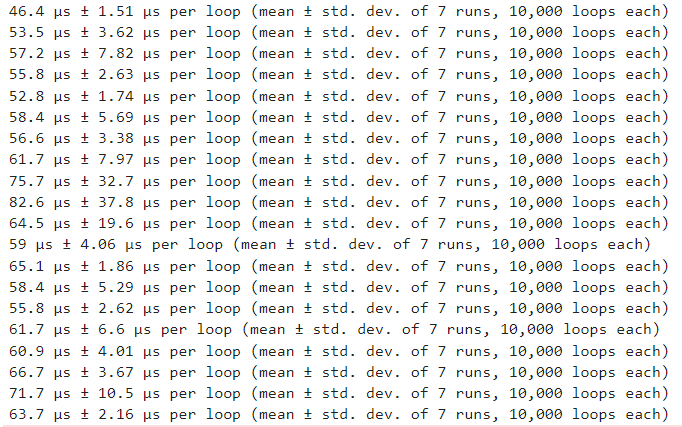
\includegraphics[width=.9\textwidth]{energy-calc.png}
    \caption{Evaluation time for arbitrary configurations with $N = 1, 2, ..., 20$}
    \label{fig:energy-calc}
\end{figure}
Similarly, calculations of energy before and after a spin flip shows a similar trend, as can be seen from the code. However, this step is implemented inside a $for-loop$, which makes it grow roughly quadratically with the number of lattice points. This step is at the heart of the \verb|Metropolis-Hastings| algorithm.\\
The critical coupling, $J_c$, gives the value of the coupling beyond which spontaneous magnetisation takes place for a given non-zero external magnetic field. This is an example of a phase transition, whose universality across different physical systems has been well studied. This can be seen from figure \ref{fig:mag-int-analy}. The value of $J_c$ is about $0.44$.\\
\begin{figure}[h!]
    \centering
    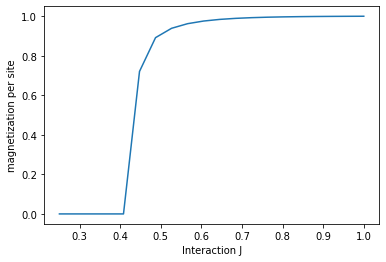
\includegraphics[width=.9\textwidth]{mag-int-analy.png}
    \caption{Analytical result for Magnetisation vs. Coupling factor}
    \label{fig:mag-int-analy}
\end{figure}



\end{document}